\chapter{Disseny e implementaci\'{o}}
\label{cha:dessign}

En aquest cap\'{i}tol veurem els patrons de dissenys emprats i les tecnologies implementades. Tamb\'{e} descriurem la interf\'{i}cie d'usuari m\'{e}s complexa i el fluxe de les operacions de sistema

\section{Esquema general arquitect\'{o}nic del sistema}
A continuaci\'{o} veiem un gr\`{a}fic amb els principals components del sistema i com es relacionen.

\begin{figure}[h]
  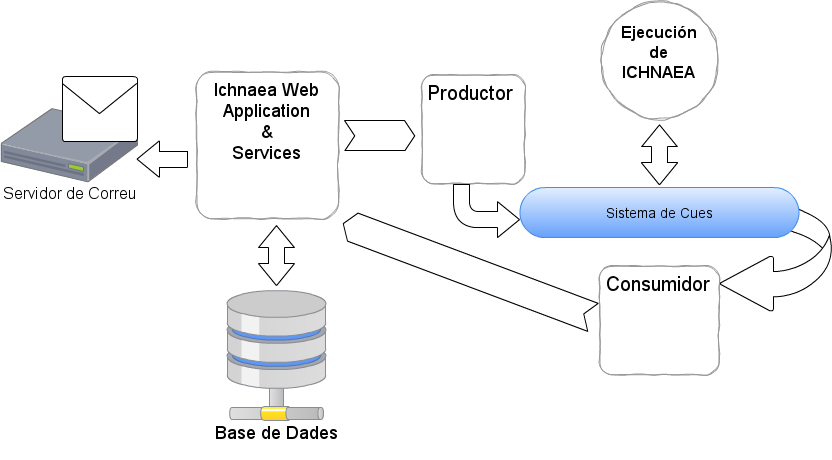
\includegraphics[scale=0.5]{img/design/ArchitectureSoftware.png}
  \caption{Arquitectura del sistema}
  \label{dessign:archsoftware}
\end{figure}
On:
\begin{itemize}
\item Ichnaea Web Application & Services \'{e}s el codi de la aplicaci\'{o} i els serveis HTTP
\item Servidor de correu \'{e}s el servidor SMTP per enviar correus electr\`{o}nics als usuaris
\item Productor-Cua-Consumidor \'{e}s el sistema de cues. Expliquem el paradigma a cap\'{i}tol \ref{dessign:queue_system_overview}. La funci\'{o} \'{e}s gestionar els inicis, fluxes i finals d'execucions de Ichnaea.
\item La base de dades on es guardan on els contiguts i models de dades i resultats.
\end{itemize}

\section{Patr\'{o} de disseny}
Per la implementaci\`{o} del sistema web s'han usat els seg\�{u}ents patrons de disseny:
  \begin{itemize}
  \item Model-Vista-Controlador amb controlador frontal
  \item Capa de Servei
  \item Injecci\'{o} de depend\`{e}ncies
  \item Repositori de model de dades
  \item Capa de mapejat de dades
  \item View template
  \item Interficies enriquides amb servei webs
  \end{itemize}

\subsection{Esquema del disseny}
\begin{figure}[h]
  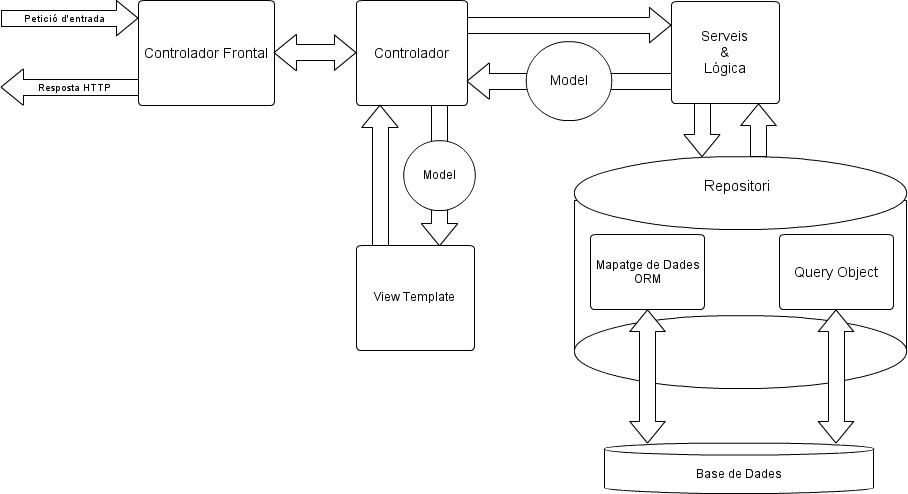
\includegraphics[scale=0.4]{img/design/IchnaeaPatterns.png}
  \caption{Patrons de disseny}
  \label{dessign:dessignpatters}
\end{figure}

Els components MVC amb controlador frontal \'{e}s un disseny t\'{i}pic en les aplicacions webs on:
\begin{itemize}
\item el model \'{e}s una representaci\'{o} de les dades en les que treballa la aplicaci\'{o}
\item la vista transforma el model a un format visible i llegible
\item el controlador frontal rep totes les peticions i les redirigeixs als controladors corresponents
\item el controlador se encarrega de processar les peticcions especifiques
\end{itemize}
L'arquitectura MVC separa la capa de presentaci\'{o} de la l\`{o}gica de domini. La capa de presentaci\'{o} accedeix a la capa de domini mitjan�ant serveis, injectant depend\'{e}ncies.EXPLICAR INJECCION DE DEPENDENCIAS\\
Els serveis, en aquest cas, contenen l\'{o}gica de Ichnaea. Accedeixen mitjan�ant les dades repositoris d'objectes. EXPLICAR REPOSITORIS i DAPAMAPPING.

\section{Implementaci\'{o} i tecnologies}
\subsection{Symfony}
Symfony2 \'{e}s un HTTP framework. Nativament implementa una variaci\'{o} del Model-Vista-Controlador amb controlador frontal amb injecci\'{o} de depencies a la capa de serveis. \\
Arquitectonicament, Symfony2 estructura el codi en Bundle, similar als paquets de JAVA. Els ''bundle'' son un conjunt de serveis, entitats i recursos independents entre si. Els bundles implementats son
\begin{itemize}
\item{Bundle de usuaris: UserBundle}
\item{Bundle de matrius: MatrixBundle}
\item{Bundle de trainings: TrainingBundle}
\item{Bundle de serveis webs: ApiBundle}
\item{Bundle de predicci\'{o}: PredictionBundle}
\end{itemize}

\subsection{Recursos}
La estructura de recursos de la aplicaci\'{o} \'{e}s la seg\�{u}ent:\\
\begin{itemize}
\item Matrius: matrix/\{id\}/
\item ''Trainings'': matrix/\{id\}/training/\{id\}
\item ''Predctions'':matrix/\{id\}/training/\{id\}/prediction/\{id\}
\end{itemize}
S'ha emprat aquesta estructura de recursos degut a les depencies entre les diferentes entitats. Un training depen d'una matriu i una predicci\'{o} depen d'un ''training''.

\section{Servei web}
S'ha desenvolupat una llibreria API JSON Restful per enriquir les interficies. S'ha emprat aquesta tecnologia per la escalabilitat que aporta i perque en un futur es pogui aprofitar el desenvolupament d'aquesta.
Les operacions, els recursos i el parametres son:\\

\begin{tabular}{ | l | p{5cm} |}
\hline
GET & /api/season/(id) \\ \hline
POST & /api/season/searchByName \\ \hline
GET & /api/variable/(id)/seasonSet \\ \hline
DELETE & /api/variable/(id)/seasonSet/(id)\\ \hline
DELETE & /api/variable/(id)/seasonSet/(id) /component/(id) \\ \hline
DELETE & /api/variable/(id)/seasonSet/(id) /component/(id)/complete\\ \hline
PUT & /api/matrix/(id)/column/(id)\\ \hline
PUT & /api/matrix/(id)/sample/(id)\\ \hline
\end{tabular}

\section{Integraci\'{o} amb el sistema de cues RabbitMQP}
\subsection{Introducci\'{o} a l'arquitectura de cues}
\label{dessign:queue_system_overview}
PETIT DIAGRAMA I EXPLICACI\'{O} DE CONSUMIDORS I PRODUCTORS
\subsection{Consumidors}
\subsubsection{Consumidor ''trainings''}
\subsubsection{Consumidor de prediccions}

\section{Interf\'{i}cies}
\subsection{Interf\'{i}cie de configuraci\'{o} de matrius}
\subsection{Interficies de carrega de matrius per fitxers }



